\documentclass[11pt]{article}

\usepackage[T1]{fontenc}
\usepackage{lmodern}
\usepackage[htt]{hyphenat}
\usepackage[margin=1in]{geometry}
\usepackage{amsmath,amssymb,amsthm}
\usepackage{booktabs}
\usepackage{array}
\usepackage{microtype}
\usepackage[numbers,sort&compress]{natbib}
\usepackage[hidelinks]{hyperref}
\usepackage{pgfplots}
\pgfplotsset{compat=1.18}
\usetikzlibrary{positioning, decorations.pathreplacing}

\newtheorem{proposition}{Proposition}
\newtheorem{definition}{Definition}

\title{Decoder-Recoverable Is Not Communicable:\\
One-Clue Reference Under Constrained Vocabularies}
\author{Brian H. Liou\\\small Independent Researcher\thanks{Contact: \texttt{brian@brianhliou.com}. Preprint; comments welcome.}}
\date{June 2026}

\begin{document}
\maketitle

\begin{abstract}
Cooperative word-association games such as Codenames pose a problem of
constrained reference: a speaker indicates a hidden subset of a 25-word board to
a partner using one legal word and a count. We ask whether a single clue can
reliably indicate an arbitrary nine-word subset, and decompose the question with
a six-rung model ladder separating channel capacity, embedding geometry,
vocabulary projection, and pragmatic interpretation. Under a frozen
common-English vocabulary and a deterministic embedding-rank decoder, exact
recovery of a nine-word subset is available for only $0.286\%$ of board-relative
target sets, by exact enumeration over $2.0 \times 10^{8}$ assignments, with a
practical frontier near six. The limit is not geometric: synthetic vectors
separate essentially every subset in 300 dimensions, so the wall
is the projection from an ideal separating direction onto a legal word. In
controlled pilot audits, the separations the decoder certifies do not transfer
to pragmatic receivers: language-model and blinded-human guessers recover
ordinary semantic clues at 23 of 24 but decoder-certified challenge clues at 0
of 44, a dissociation that survives stronger receivers and reproduces on natural
game distributions. The dominant variable for natural recoverability is the
availability of a clean separating concept, not the target count. A symbolic
WordNet replication reproduces the collapse with no embedding. More broadly, the
result bounds when embedding cosine similarity is a safe proxy for communication:
least so at high cardinality and low margin, the regime where it is most tempting
to trust.
\end{abstract}

\section{Introduction}

Cooperative word-association games such as Codenames pose a problem of
\emph{constrained reference}. A speaker observes a board of words, holds a hidden
target subset in mind, and must select a single legal word that causes a
receiver to identify exactly that subset. The speaker cannot point, cannot
enumerate the targets, and cannot agree on an arbitrary private code: the message
is one word from a shared vocabulary, and the receiver must recover the intended
set from meaning. This is a compact instance of a general question about
communication. How much information about a structured referent can a single
symbol carry when the channel is a shared, finite, natural vocabulary?

We study the strongest form of the question that the game admits. A board holds
25 words and a hidden target subset holds up to 9. The rules invite a tempting
move: find one clue that points at all nine targets at once and win on the first
turn. Whether such a clue reliably exists is the question we formalize and
measure. The answer turns on several constraints that are easy to conflate: the
information capacity of a one-word channel, the geometry of the embedding space
in which similarity is computed, the coverage of the legal vocabulary relative to
that geometry, and the pragmatics of how a real receiver interprets a word.

The one-word channel is much weaker than the game's nominal ceiling. Recovering
an arbitrary 9-of-25 subset takes about 21 bits while one common-English word
carries about 12.8, so no \emph{universal} one-word strategy exists; the live
question is per-instance existence. Under a frozen common-English vocabulary and
an embedding-rank decoder, exact recovery of a 9-word subset is available for
only $0.286\%$ of board-relative target sets, by exact enumeration over
$2.0 \times 10^{8}$ assignments, with a practical frontier near six. The
shortfall is not geometric: synthetic vectors separate essentially every subset
in 300 dimensions, so the wall is the \emph{projection} from an ideal direction
onto a legal word. The separations the decoder does certify then fail a second
test: in a controlled audit, receivers recovered ordinary clues at 23 of 24 but
decoder-certified clues at 0 of 44, so decoder-recoverability and communicability
come apart. What dominates natural recoverability is the availability of a clean
separating concept, not the count; both walls reproduce on natural game boards
and in a symbolic model with no embedding in it.

The result matters beyond the game. Embedding cosine similarity is a common proxy
for ``this symbol communicates this meaning,'' and the dissociation we report shows
the proxy is unsafe at the high-cardinality, low-margin regime where it is most
tempting to trust. The same structure recurs beyond the game, in retrieval and
reranking, single-word cluster labeling, caption generation, and embedding-based
evaluation; in each, optimizing the similarity score optimizes a target a human
receiver does not share. The constrained-reference framing also connects the problem to
referential and signaling games, where the gap between what a continuous
representation permits and what a discrete shared vocabulary realizes is the
object of study rather than an implementation detail.

\paragraph{Contributions.}
\begin{enumerate}
  \item A \textbf{model ladder} that decomposes one-clue communication into six
    regimes (arbitrary codebook, bounded convention, known decoder,
    embedding-rank decoder, synthetic vector, and public-concept / natural
    language), each isolating a distinct constraint, with explicit bounding
    relations between regimes.
  \item An \textbf{exact characterization and measurement} under the
    known-decoder embedding-rank model: universal first-turn-9 is false
    ($0.286\%$ coverage), the practical exact frontier is near six, and the
    limit is vocabulary projection rather than embedding geometry.
  \item A \textbf{dissociation result with positive controls}: clues that are
    certified exact recoveries under the embedding decoder do not transfer to
    pragmatic receivers (0 of 44), while ordinary semantic clues do (23 of 24);
    a stronger receiver tier replicates the zeros.
  \item \textbf{Identification of the dominant variable} for natural
    recoverability: clean cluster availability, with target count secondary, and
    a threshold-like collapse at the first same-category distractor; the collapse
    replicates on natural random-game distributions, where cluegivers free to
    choose their own move retreat to counts 1 through 3.
  \item A \textbf{non-embedding replication} over symbolic WordNet concepts that
    reproduces the same high-count collapse, defending the central claim against
    a purely embedding-geometric reading.
\end{enumerate}

\section{Related Work}\label{sec:related}

\subsection{Codenames as an AI Benchmark}

The Codenames AI line begins with \citet{kim2019cooperation}, which introduced
the competition setup, agents built on WordNet and word2vec/GloVe similarity, and
paired and unknown-teammate evaluation. Later agent work extended the cluegiver
and guesser roles with transformer and word-association methods
\citep{jaramillo2020word} and with language graphs and embedding scoring for
multi-target clue generation \citep{koyyalagunta2021playing}. A
strategic-reasoning thread models the partner explicitly: recursive teammate
modeling \citep{bills2023deductive}, adaptation under partner uncertainty
\citep{archibald2024adapting}, semantic-noise modeling
\citep{archibald2024noisy}, and Bayesian inference over partner pragmatics within
a cognitive hierarchy \citep{bills2025cooperation}. A recent strand evaluates
large language models directly, framing Codenames as an LLM benchmark
\citep{stephenson2024codenames} and as ad-hoc concept formation over target words
\citep{hakimov2025adhoc}. Human and cross-cultural play is studied through
Codenames Duet \citep{shaikh2023modeling, white2024communicate}, and a visual
analogue appears in WinoGAViL \citep{bitton2022winogavil}.

These works build agents and measure their performance. None characterizes which
target subsets are recoverable from one clue, or separates the reasons a
high-count clue fails. This paper supplies that map.

\subsection{Pragmatics and Decoder-Aware Speakers}

Our known-decoder model, where the cluegiver knows exactly how the partner will
interpret a clue, is an instance of a speaker who chooses words by modeling the
listener. The Rational Speech Acts framework \citep{frank2012predicting}
formalizes that recursion; neural versions rerank utterances against a learned
listener \citep{andreas2016pragmatics}; and signaling-game theory
\citep{lewis1969convention, skyrms2010signals} supplies the language of learned
sender/receiver conventions. These describe \emph{how} such a speaker should
choose. None quantifies, for a fixed board and vocabulary, \emph{which} target
subsets it can actually reach.

\subsection{Separability and Learning Theory}

The synthetic-vector upper bound rests on classical separability results. Cover's
function-counting theorem \citep{cover1965geometrical} counts the linearly
separable dichotomies of points in general position and underwrites
Proposition~\ref{prop:geometry}; linear-separability and convex-hull
characterizations give the geometric condition for a clue direction to separate
targets from distractors. Several tools sharpen the failure side: VC dimension
and the Sauer-Shelah lemma bound how many board subsets a vocabulary-plus-decoder
concept class can realize, and separating / cover-free families and teaching
dimension frame a clue vocabulary as a set system that must distinguish subsets
with few messages. These results bound geometry and capacity in the abstract;
they do not predict which natural clues a real vocabulary realizes, which is the
projection question Section~6.3 measures.

\subsection{Semantic Communication}

The semantic-communication literature reframes communication around task success
and meaning rather than bit-exact recovery, positioning the problem beyond
Shannon channel capacity. It motivates the distinction between
decoder-recoverability and communicability without supplying a board-specific
feasibility result.

\subsection{Gap}

Existing work offers Codenames agents and benchmarks, pragmatic speaker/listener
models, partner-adaptation and noisy-communication variants, and general
separability and learning-theory tools. The object none supplies is a
board-relative, decoder-explicit characterization of which hidden target subsets
are recoverable from one constrained semantic clue, with feasibility curves by
target count and failure modes that separate information, geometry, vocabulary,
and receiver limits. That is the contribution of this paper.

\section{Problem Formulation}\label{sec:problem}

\subsection{One-Clue Recoverability}

Let $B = \{w_1, \dots, w_n\}$ be a board of $n$ distinct words. A hidden target
subset $T \subseteq B$ has size $|T| = k$. A cluegiver transmits a message $c$
from a legal message set $V$ together with a count $k$. A decoder $D$ maps the
board, message, count, and public history $H$ to an ordered list of guesses:
\[
  D(B, c, k, H) = (g_1, g_2, \dots, g_n), \qquad g_i \in B \text{ distinct.}
\]

\begin{definition}[one-clue recoverability]
A target subset $T$ is one-clue recoverable under $(B, V, D, H, k)$ if there
exists a legal message $c \in V$ such that the first $k$ guesses returned by the
decoder are exactly the targets:
\[
  \{ g_1, \dots, g_k \} = T,
\]
where $(g_1, \dots, g_k)$ is the length-$k$ prefix of $D(B, c, k, H)$.
\end{definition}

The first-turn instance fixes $n = 25$, the empty history $H = \emptyset$, and
the target count $k$ (with $k = 9$ the headline case).

Two distinct quantities follow from this definition, and conflating them is the
source of most confusion about the game's difficulty:
\begin{itemize}
  \item \textbf{Per-instance existence.} For a given board and target subset
    $(B, T)$, does any legal $c \in V$ recover $T$?
  \item \textbf{Universal guarantee.} Does a single protocol recover \emph{every}
    $k$-subset of \emph{every} board?
\end{itemize}
The universal guarantee is settled cheaply by counting (Section~\ref{sec:bounds}).
The per-instance question is the one that decides whether the first-turn-9
strategy is real, and it is the question the empirical sections answer.

\subsection{The Model Ladder}

The recoverability of a subset depends entirely on what counts as a legal message
and how the receiver decodes it. We organize the assumptions into a ladder of
models, ordered from the loosest channel to the most faithful account of human
play. Two rungs are idealized bounds rather than playable models, and we mark
them as such. For a fixed board and target space, write $R_M$ for the set of
target subsets recoverable under model $M$; the bounding relations below are
stated in terms of $R_M$.

\paragraph{(1) Codebook model.}
The message set $V$ is an arbitrary set of pre-agreed codewords carrying a private
bijection to target subsets. Recoverability is limited only by channel size:
every $k$-subset is recoverable once $|V| \ge \binom{n}{k}$. This rung isolates
\textbf{raw channel capacity} and serves as the top bound,
$R_{\mathrm{codebook}} \supseteq R_M$ for every other $M$. It is a boundary case,
not a semantic model.

\paragraph{(2) Bounded-convention model.}
A legal clue word is augmented by a pre-agreed side channel of $b$ bits, giving
capacity $|V_{\mathrm{word}}| \cdot 2^b$. The rung isolates \textbf{how much
non-semantic convention} must be added to a single word to close the gap to the
codebook bound, and it interpolates between meaning-bearing clues and arbitrary
codes.

\paragraph{(3) Known-decoder model.}
The cluegiver knows the receiver's deterministic decoding algorithm $D$ and may
search the entire legal vocabulary. The recoverable set is exactly the image of
the vocabulary under the decoder,
\[
  R_{\mathrm{known}} = \{ D_k(B, c, H) : c \in V \},
\]
which is finite and enumerable. This rung isolates \textbf{what a
vocabulary-bound but receiver-omniscient speaker can achieve}, and it is the
regime relevant to AI play, where a cluegiver can simulate its partner exactly.

\paragraph{(4) Embedding-rank model.}
A concrete known decoder. The decoder ranks board words by cosine similarity
between the clue embedding and each board-word embedding and returns the top $k$:
\[
  \mathrm{score}(c, w) = \cos\!\big( \mathrm{embed}(c), \mathrm{embed}(w) \big),
\]
\[
  T \text{ recoverable} \iff
  \min_{t \in T} \mathrm{score}(c, t) > \max_{r \in B \setminus T} \mathrm{score}(c, r)
  \quad \text{for some legal } c \in V.
\]
This rung isolates the \textbf{realizable separations of a specific, widely used
similarity decoder} over a legal vocabulary. It is the headline model of the
paper.

\paragraph{(5) Synthetic-vector model.}
The message may be any vector in the embedding space, not restricted to the
embedding of a legal word. Because every legal word's embedding is itself an
admissible vector, this rung upper-bounds the embedding-rank model:
$R_{\mathrm{embed}} \subseteq R_{\mathrm{synthetic}}$. It isolates \textbf{pure
geometry}, the separations the space permits independent of vocabulary. The gap
$R_{\mathrm{synthetic}} \setminus R_{\mathrm{embed}}$ is precisely the
\textbf{vocabulary-projection loss}, and measuring that gap is the mechanism
claim of Section~\ref{sec:results}.

\paragraph{(6) Public-concept and natural models.}
The most faithful accounts of human play. In the \textbf{public-concept
extension} model, the clue names a public concept (a category tag or an ontology
node) and the receiver selects every board word in that concept's board-relative
extension; exact recovery requires the extension to contain no non-targets. We
instantiate it two ways, with word-pack category tags and with WordNet hypernym
synsets. In the \textbf{natural / pragmatic} model, the clue must work by
ordinary meaning for a human or language-model receiver. The pragmatic model is
the hardest to formalize; we approximate it with controlled language-model audits
and reserve human panels for later validation. These rungs are not strictly
nested with the embedding-rank model: a clue can be naturally communicable yet
decoder-unrecoverable, and the converse, which is the dissociation the paper
reports.

The ladder gives the paper its spine (Figure~\ref{fig:ladder}). Rungs (1) and (5) are upper bounds that
establish that neither channel capacity nor geometry is the limiting factor.
Rungs (3) and (4) localize the constraint to vocabulary projection. Rung (6) is
the target the whole construction is meant to explain, and it is where
decoder-recoverability and communicability separate.

\begin{figure}[t]
\centering
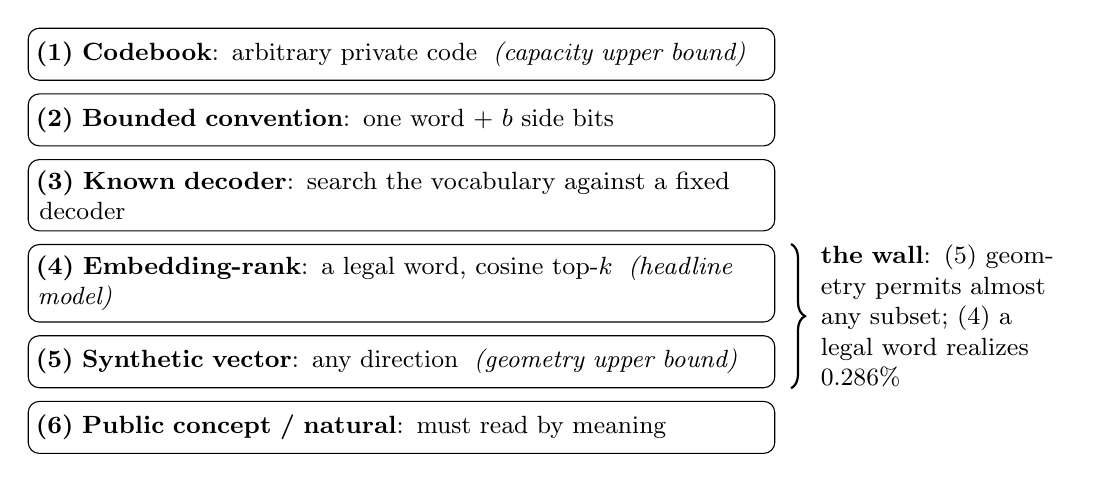
\begin{tikzpicture}[font=\small,
  rung/.style={draw, rounded corners, text width=9.2cm, minimum height=0.66cm, align=left, inner sep=4pt},
]
\node[rung] (r1) {\textbf{(1) Codebook}: arbitrary private code \;\textit{(capacity upper bound)}};
\node[rung, below=1.6mm of r1] (r2) {\textbf{(2) Bounded convention}: one word $+$ $b$ side bits};
\node[rung, below=1.6mm of r2] (r3) {\textbf{(3) Known decoder}: search the vocabulary against a fixed decoder};
\node[rung, below=1.6mm of r3] (r4) {\textbf{(4) Embedding-rank}: a legal word, cosine top-$k$ \;\textit{(headline model)}};
\node[rung, below=1.6mm of r4] (r5) {\textbf{(5) Synthetic vector}: any direction \;\textit{(geometry upper bound)}};
\node[rung, below=1.6mm of r5] (r6) {\textbf{(6) Public concept / natural}: must read by meaning};
\draw[decorate, decoration={brace, amplitude=5pt}, thick]
  ([xshift=2mm]r4.north east) -- ([xshift=2mm]r5.south east)
  node[midway, right=7pt, text width=3cm] {\textbf{the wall}: (5) geometry permits almost any subset; (4) a legal word realizes $0.286\%$};
\end{tikzpicture}
\caption{The model ladder, from the loosest channel (top) to the most faithful
account of human play (bottom). Rungs (1) and (5) are idealized upper bounds, not
playable models: neither channel capacity nor geometry forbids a first-turn-nine
clue. The vocabulary-projection wall is the gap between rungs (5) and (4): a
separating direction exists for almost any subset, but a legal word realizes one
for only $0.286\%$ of nine-subsets (Sections~6.1--6.3).}
\label{fig:ladder}
\end{figure}

\section{Theoretical Bounds}\label{sec:bounds}

Four facts bound the problem before any measurement. The first settles the
universal question and isolates per-instance existence as the one that remains.
The second makes per-instance existence computable. The third states the exact
recovery condition for the embedding-rank decoder. The fourth establishes that
geometry is permissive, which localizes the limit to the vocabulary.
Throughout, $n$ is the board size and $k$ the target count, with the headline
case $n = 25$, $k = 9$.

\subsection{The Information-Theoretic Floor}

\begin{proposition}[pigeonhole]\label{prop:pigeonhole}
Any single-message protocol that guarantees exact recovery of every $k$-subset of
an $n$-word board requires at least $\binom{n}{k}$ distinguishable messages.
\end{proposition}

\begin{proof}
Distinct target subsets must map to distinct messages; if two subsets share a
message, at least one is not recovered. There are $\binom{n}{k}$ subsets.
\end{proof}

For the headline case, $\binom{25}{9} = 2{,}042{,}975$, equivalently
$\log_2 \binom{25}{9} \approx 20.96$ bits. A single word drawn from the
Brown-common vocabulary of 7,009 legal clues provides at most
$\log_2 7009 \approx 12.78$ bits when treated as a uniform symbol channel, a
deficit of about 8.19 bits. No single common-English word can serve as a
universal first-turn-9 protocol: by capacity alone, one word cannot distinguish
the required number of subsets.

This bound concerns the \emph{universal} guarantee. It says nothing about whether
a \emph{given} target subset admits a recovering clue. The per-instance existence
question survives Proposition~\ref{prop:pigeonhole} untouched, and it is the
question the rest of the paper answers.

\subsection{Decoder-Image Enumerability}

\begin{proposition}\label{prop:image}
For a fixed board $B$, finite legal vocabulary $V$, deterministic decoder $D$,
history $H$, and count $k$, the recoverable target subsets are exactly the image
of the vocabulary under the decoder,
\[
  R_{\mathrm{known}} = \{ D_k(B, c, H) : c \in V \},
\]
and $|R_{\mathrm{known}}| \le \min\!\big( |V|, \binom{n}{k} \big)$.
\end{proposition}

\begin{proof}
The map $c \mapsto D_k(B, c, H)$ is a function from $V$ into the $k$-subsets of
$B$. The recoverable subsets are its image, whose size is at most the size of the
domain $|V|$ and at most the size of the codomain $\binom{n}{k}$.
\end{proof}

Two consequences follow. First, recoverability under any known deterministic
decoder is decidable by enumeration: evaluate $D$ on every legal clue and collect
the decoded subsets. This is what makes the coverage figure in Section~6.2 an
exact count rather than an estimate. Second, the bound is usually loose from
below, because many clues decode to the same subset, so the realized image is far
smaller than $|V|$. The measured coverage quantifies how much smaller.

\subsection{Rank Separability}

\begin{proposition}\label{prop:rank}
Under the embedding-rank decoder, a clue $c$ gives a tie-free recovery
certificate for target subset $T$ when every target outscores every non-target,
\[
  m(c, T) := \min_{t \in T} \mathrm{score}(c, t)
             - \max_{r \in B \setminus T} \mathrm{score}(c, r) > 0,
\]
and $c$ certifies non-recovery when $m(c, T) < 0$. At the boundary
$m(c, T) = 0$, recovery depends on the decoder's fixed tie-breaking rule. Thus
$\max_{c \in V} m(c, T) > 0$ certifies recoverability over $V$, while
$\max_{c \in V} m(c, T) < 0$ certifies non-recoverability.
\end{proposition}

\begin{proof}
The decoder returns the top $k$ board words by score. If all $k$ targets score
strictly above all $n - k$ non-targets, the length-$k$ prefix is exactly $T$. If
a non-target scores strictly above at least one target, $T$ cannot be the
length-$k$ prefix. Exact score ties at the boundary are determined by the
decoder's fixed tie-breaking rule.
\end{proof}

The quantity $\max_{c \in V} m(c, T)$ is the \textbf{projection margin} of a
target subset. A positive projection margin certifies recoverability without
relying on ties; a negative projection margin certifies non-recoverability
because no legal clue separates $T$ from the board. Section~6.2 reports such
negative certificates directly, including a $k = 9$ subset whose best legal clue
still leaves a margin of $-0.069$.

\subsection{The Geometry Upper Bound}

\begin{proposition}[synthetic separability]\label{prop:geometry}
If the $n$ board vectors are in general position and $n \le d + 1$, where $d$ is
the embedding dimension, then for every target subset $T$ there exists a query
vector $v$ ranking all of $T$ above all of $B \setminus T$. Equivalently,
$R_{\mathrm{synthetic}}$ is the full set of $k$-subsets.
\end{proposition}

Because the decoder ranks board words by cosine, the relevant points are the
\emph{unit-normalized} board vectors: ranking by $\cos(v, e_w)$ is ranking by the
dot product of $v$ with $e_w / \|e_w\|$. The embedding packs store L2-normalized
vectors (Section~5.1), so the general-position condition is stated, and checked,
on exactly the vectors the decoder ranks.

\begin{proof}[Justification]
Points in general position in dimension $d$ are linearly separable under any
binary labeling once $n \le d + 1$; Cover's function-counting theorem counts the
affinely separable dichotomies of $n$ points in general position, and for
$n \le d + 1$ the count is all $2^n$ labelings. The separating hyperplane's
normal induces a score direction, and the separating threshold witnesses that
every target receives a higher score than every non-target. The threshold is only
a proof device; it is not sent to the decoder. For $n = 25$ and $d = 300$ the
condition holds with wide margin, and we confirm affine independence of the
embedded board vectors on 100 of 100 sampled boards per pack (Section~6.1).
\end{proof}

Every legal word's embedding is itself an admissible query vector, so the
synthetic model upper-bounds the embedding-rank model:
$R_{\mathrm{embed}} \subseteq R_{\mathrm{synthetic}}$.
Proposition~\ref{prop:geometry} makes $R_{\mathrm{synthetic}}$ essentially
complete, so the embedding-rank shortfall measured in Section~6.2 cannot be
attributed to geometry. The gap
$R_{\mathrm{synthetic}} \setminus R_{\mathrm{embed}}$ is exactly the set of
subsets whose separating direction exists but is realized by no legal word: the
vocabulary-projection loss that Section~6.3 isolates.

\section{Experimental Setup}\label{sec:setup}

\subsection{Boards, Vocabulary, and Decoder}

The setup has three independent pieces, each with its own pack: the \emph{boards}
(the 25 words shown), the \emph{clue vocabulary} (the legal one-word guesses), and
the \emph{embedding} (the vectors). They are distinct; in particular the
7,009-word vocabulary below is the set of legal clues, not the boards, and the
coverage figures enumerate every target subset of a board rather than sampling
boards.

Boards are drawn from two packs of concrete English nouns. The primary pack is
\texttt{wordnet-concrete-v0.1}; a second pack,
\texttt{wordnet-concrete-band2-v0.1}, drawn from a disjoint frequency band,
serves as a board-distribution sensitivity check. Each board holds 25 words, and
target counts range over $k = 1..9$.

The legal clue vocabulary is \texttt{wordnet-brown-common-v0.1}, 7,009 words. It
is constructed from exact WordNet lemmas filtered by a Brown-corpus frequency
floor and intersected with the embedding pack, so every legal clue is a
common-English word with a known vector. It is a reproducible common-English
tier, not a claim about any official tabletop dictionary. Two looser tiers, a
permissive lexical set and a WordNet-common set, are used only as ablations in
Section~6.3.

The primary embedding is \texttt{glove-6B-300d-slim}, the 300-dimensional GloVe
vectors restricted to the working vocabulary. Vectors are L2-normalized when the
pack is built, so cosine similarity is computed as a dot product and every
geometric statement in Section~\ref{sec:bounds} refers to the unit-normalized
vectors the decoder actually ranks. The decoder is the deterministic
embedding-rank decoder of Section~3.2: score every board word by cosine
similarity to the clue and return the top $k$, with a fixed tie-break. Embedding
dependence is checked with a second distributional source,
\texttt{glove-840B-300d-case-agg-slim}, built from Common Crawl GloVe-840B by
aggregating cased variants into lowercase forms, and with the symbolic
non-embedding replication in Section~6.7.

A small coverage caveat applies to the primary embedding. Two pack-1 words and
six pack-2 words have no \texttt{glove-6B} vector; a board containing such a word
is scored over its embedded words only, so its assignment space is
$\binom{24}{k}$ or $\binom{23}{k}$ rather than $\binom{25}{k}$. Concretely, 97 of
100 pack-1 boards have all 25 words embedded and 3 have 24; for pack 2 the split
is 87 / 11 / 2 boards with 25 / 24 / 23 embedded words. All denominators in
Section~\ref{sec:results} count assignments over the embedded words per board.
The second embedding covers every pack word, so its boards are all 25 words; the
small difference in effective board size is noted where the two embeddings are
compared (Section~\ref{sec:limitations}).

\subsection{The Pragmatic Audit Protocol}

Whether a clue communicates to a real reader is not something we can compute the
way we compute the embedding decoder: the natural / pragmatic model of
Section~3.2 has no formula. So we approximate
a pragmatic receiver with large-language-model guessers, used as a stand-in for
human receivers pending an independent human panel (Section~\ref{sec:conclusion}),
plus a blinded single-judge human author-pilot over a stratified 72-item packet
(Section~6.4). A guesser sees the board, a clue, and a count, and returns an
ordered list of guesses under the same recovery criterion as the decoder. Two
small-tier models run each audit queue, \texttt{gpt-5.4-nano} and
\texttt{claude-haiku-4-5}, with the cluegiver and guesser blinded to each other;
the controls-and-challenge queue is additionally rerun with two stronger
receivers, \texttt{gpt-5.4} and \texttt{claude-sonnet-4-6}, as a
receiver-capability check (Section~6.4).

Every audit queue mixes two item classes. \textbf{Positive controls} are ordinary
semantic clues over clean categories (for example \texttt{animal 3},
\texttt{vehicle 4}); they verify that the protocol recovers clues a competent
receiver should get. \textbf{Challenge items} come from the embedding-rank
decoder's frontier and counterexample searches, and they split by certification
status: 44 items carry a positive projection margin, meaning the decoder provably
recovers the declared subset from that clue, and 20 items carry a negative margin,
the best available legal clue for a subset the decoder cannot recover. Only the 44
certified items bear on the dissociation claim; the 20 negative-margin items are
reported separately as near-threshold contrasts. Frontier items declare the count
of the decoder-certified subset: for 20 of the 40 frontier items that subset is a
proper contained subset (counts 4 through 7) of a 9-target key, and exact recovery
is scored against the certified subset, which is what the clue provably indicates
under the decoder. The controls are the load-bearing methodological check. If the
guessers failed them, the audit prompt would be suspect; they do not. The guesser
prompt contains only the board words, the clue, and the count; targets are never
included.

Two bridge designs ground the audits in the game's natural distribution
(Section~6.6). The \emph{stratified random-game queue} samples real first-turn
boards and hidden keys under the standard ruleset and draws one target subset per
count 4--9 per board from the actual key. The \emph{best-move queue} shows the
cluegiver the full 9-target key and lets it choose its own clue, count, and
intended subset; generated moves are legality-filtered (single non-board clue
word, chosen subset within the key, count matching the subset) before blinded
audit, and exact recovery is scored against the cluegiver's own declared subset.

Two metrics are reported. \textbf{Exact recovery} is the fraction of items where
the first $k$ guesses equal the target set. \textbf{Target-hit rate} is the
fraction of all guesses that fall on targets, a partial-credit measure that
separates ``wrong set'' from ``no idea.''

\subsection{Statistics}

Each result is labeled by how it was computed, and the paper uses three
computation classes.

\paragraph{Exact counts.}
The headline coverage figure (Section~6.2) is exact, not sampled: by
Proposition~\ref{prop:image} the recoverable set is the decoder image over the
7,009-word vocabulary, so coverage is an exact count over all board-relative
target assignments. The symbolic public-concept rates of Section~6.7 are also
exact, computed by inclusion-exclusion over board-relative concept extensions.

\paragraph{Sampled estimates.}
The first-turn frontier tables (Sections~6.2 and~\ref{sec:limitations}) sample
1,000 random 9-target keys per board (100,000 per pack), and the vocabulary-tier
projection table (Section~6.3) samples 1,000 subsets per count per board. These
are estimates with sampling error of order $\pm 0.003$ on rates near 0.5 and
$\pm 0.0002$ on rates near 0.003 (one standard error). In particular, the
frontier's sampled $P(=9)$ and the exact coverage rate estimate the same quantity
under uniform random keys; any small disagreement between them is sampling error,
not a model difference.

\paragraph{Pilot counts.}
The language-model audits are pilot-scale; every audit table reports raw counts
and is labeled as a pilot where the per-cell sample is small. We do not attach
confidence intervals to the audit rates; the 0-of-44 and 23-of-24 contrasts are
reported as observed counts.

\section{Results}\label{sec:results}

The results run as one argument. The upper-bound rungs of the ladder are
permissive, so neither channel capacity nor geometry is the constraint (6.1).
Under a realistic decoder, the universal first-turn-9 strategy collapses (6.2).
The collapse is a vocabulary effect, not a geometry effect (6.3). The separations
the decoder does certify fail to reach pragmatic receivers (6.4). What dominates
pragmatic recoverability is clean concept separation, with target count secondary
(6.5). The collapse reproduces on natural random-game distributions, where
cluegivers free to choose their own move retreat below the frontier (6.6). A
symbolic, non-embedding model reproduces the same shape (6.7).

\subsection{The Upper Bounds Are Permissive}

\textbf{Neither channel capacity nor geometry forbids first-turn-9.} The codebook
rung makes every 9-subset recoverable once the channel carries the 2,042,975
messages of Proposition~\ref{prop:pigeonhole}, so the problem is not impossible in
principle. The synthetic-vector rung makes it geometrically available: across 100
sampled boards per pack, the embedded board vectors (25 per board on most boards;
24 on three pack-1 boards and 23--24 on thirteen pack-2 boards, per the coverage
caveat of Section~5.1) were affinely independent in 100 of 100 cases for each
pack, so by Proposition~\ref{prop:geometry} a separating query direction exists
for essentially every target subset. The interesting failure therefore lives
strictly between ``any vector'' and ``a legal word.''

\emph{Caveat.} General position is a property of the sampled GloVe boards; a
degenerate embedding could in principle violate it, which is why the condition is
checked rather than assumed.

\subsection{Universal First-Turn-9 Collapses Under a Realistic Decoder}

\textbf{Under a frozen common vocabulary and the embedding-rank decoder, almost no
9-subset is recoverable.} Exact enumeration over the decoder image gives a
$k = 9$ coverage of $578{,}424 / 202{,}091{,}087 = 0.286\%$ on the primary pack:
fewer than three in a thousand board-relative 9-subsets admit any legal
recovering clue. The denominator counts 9-subsets of the embedded words per
board: 97 boards contribute $\binom{25}{9}$ and three contribute $\binom{24}{9}$
(Section~5.1). A direct certificate makes the failure concrete. On a 25-word
board with targets \texttt{\{barn, builder, call, colonel, educator, pit,
product, specialist, wood\}}, the best legal clue (\texttt{darling}) still leaves
a projection margin of $-0.069$, so by Proposition~\ref{prop:rank} no legal clue
separates the set. The certificate is a statement about the explicit board word
list recorded in the artifact (the board was drawn from an earlier revision of
the word pack); it was rechecked against the current legal vocabulary, 6,869
legal clues for that board, with the same best clue and margin.

The practical frontier sits near six. Given a random 9-target key (1,000 sampled
keys per board, 100,000 per pack; sampled estimate, Section~5.3), the largest
exactly recoverable contained subset has the following distribution:

\begin{center}
\begin{tabular}{lrrrrr}
\toprule
pack & $E[\text{best exact count}]$ & $P(\ge 6)$ & $P(\ge 7)$ & $P(\ge 8)$ & $P(=9)$ \\
\midrule
\texttt{wordnet-concrete-v0.1}       & 5.87 & 0.642 & 0.221 & 0.038 & 0.0030 \\
\texttt{wordnet-concrete-band2-v0.1} & 5.91 & 0.666 & 0.235 & 0.041 & 0.0032 \\
\bottomrule
\end{tabular}
\end{center}

The exact frontier is usually five or six, occasionally seven or eight, and rarely
nine. The sampled $P(=9)$ column and the exact coverage rate above estimate the
same quantity; they agree within sampling error.

\emph{Caveat.} The coverage figure is exact and the frontier rows are sampled
estimates, in both cases for one embedding and two board packs; generalization to
other embeddings is addressed in 6.7 and Section~\ref{sec:limitations}.

\subsection{The Bottleneck Is Vocabulary Projection}

\textbf{The collapse is the gap between what the geometry permits and what a legal
word realizes.} Synthetic vectors recover essentially everything (6.1); legal
words recover 0.286\% at $k = 9$ (6.2). The difference,
$R_{\mathrm{synthetic}} \setminus R_{\mathrm{embed}}$, is the set of subsets whose
separating direction exists but is named by no legal clue. Tightening the
vocabulary deepens the collapse monotonically; since the geometry is identical
across tiers, the effect is lexical (Figure~\ref{fig:coverage}; sampled positive-margin rates,
1,000 subsets per count per board; Section~5.3):

\begin{center}
\begin{tabular}{lrrr}
\toprule
clue tier & $k{=}3$ recoverable & $k{=}5$ recoverable & $k{=}9$ recoverable \\
\midrule
permissive lexical  & 0.932 & 0.242 & 0.0113 \\
WordNet common      & 0.689 & 0.105 & 0.0042 \\
WordNet Brown common & 0.549 & 0.072 & 0.0029 \\
\bottomrule
\end{tabular}
\end{center}

Each step toward a stricter, more natural vocabulary removes recoverable subsets,
most sharply at high counts. Simple static remedies do not change the high-count
picture: an all-but-the-top-component transform raises low-$k$ coverage but leaves
$k = 9$ near 0.003 on both packs. The wall is lexical coverage of the embedding's
separating directions, and it cannot be transformed away while the clue must be a
legal word.

\emph{Caveat.} The permissive-lexical tier is an optimistic ablation, not a
playable clue model; it bounds the effect of vocabulary loosening rather than
describing real play.

\begin{figure}[t]
\centering
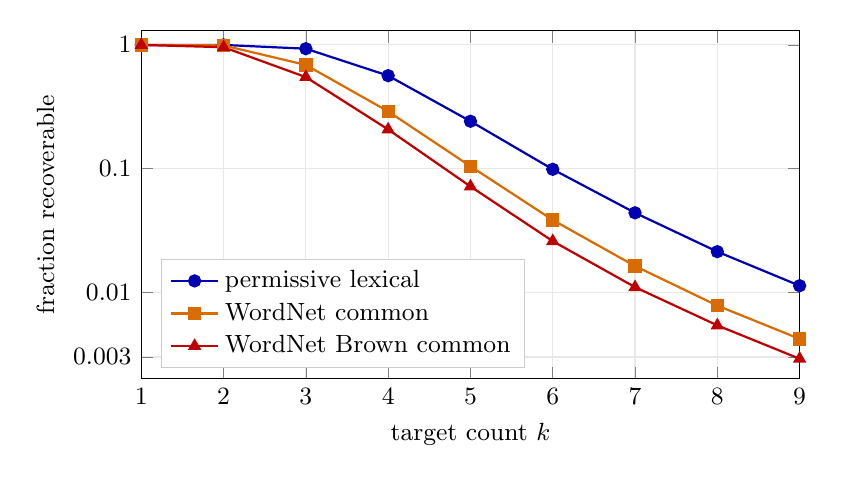
\begin{tikzpicture}
\begin{axis}[
  width=0.82\linewidth, height=6cm,
  xlabel={target count $k$}, ylabel={fraction recoverable},
  ymode=log, log basis y={10},
  xmin=1, xmax=9, ymin=0.002, ymax=1.3,
  xtick={1,2,3,4,5,6,7,8,9},
  ytick={1,0.1,0.01,0.003}, yticklabels={$1$,$0.1$,$0.01$,$0.003$},
  legend pos=south west, legend cell align=left, legend style={font=\small, draw=gray!40},
  grid=major, grid style={gray!18},
  tick label style={font=\small}, label style={font=\small},
]
\addplot[mark=*, thick, blue!70!black] coordinates {(1,1.0)(2,0.9999)(3,0.9323)(4,0.5643)(5,0.2415)(6,0.0987)(7,0.0439)(8,0.0213)(9,0.0113)};
\addlegendentry{permissive lexical}
\addplot[mark=square*, thick, orange!85!black] coordinates {(1,1.0)(2,0.9911)(3,0.6887)(4,0.2901)(5,0.1045)(6,0.0384)(7,0.0163)(8,0.0078)(9,0.0042)};
\addlegendentry{WordNet common}
\addplot[mark=triangle*, thick, red!75!black] coordinates {(1,1.0)(2,0.9586)(3,0.5492)(4,0.2072)(5,0.0717)(6,0.0259)(7,0.0110)(8,0.0054)(9,0.0029)};
\addlegendentry{WordNet Brown common}
\end{axis}
\end{tikzpicture}
\caption{Coverage collapses with target count, and a stricter vocabulary lowers
the whole curve. Fraction of board-relative target subsets a legal clue can
separate (positive projection margin) by count $k$, for three clue-vocabulary
tiers, primary pack, log scale. The common-English tier reaches $0.0029$ at
$k=9$ (the $0.286\%$ headline); each step toward a more natural vocabulary is the
projection effect of this section.}
\label{fig:coverage}
\end{figure}

\subsection{Clues Optimal Under the Decoder Do Not Reach Pragmatic Receivers}

\textbf{Decoder-recoverability and natural communicability come apart.} In the
controlled audit, language-model guessers recovered ordinary clues nearly
perfectly and recovered decoder-certified challenge clues at zero. The challenge items split by
certification status (Section~5.2): the 44 decoder-certified items
each carry a positive projection margin, so the decoder provably recovers the
declared subset from the clue, and they are the items that bear on the
dissociation; the 20 negative-margin items are near-threshold contrasts:

\begin{center}
\begin{tabular}{lcrr}
\toprule
item class & projection margin & exact recovery & target-hit rate \\
\midrule
positive controls & --- & 23/24 & 98.9\% \\
decoder-certified challenge & $+0.0001$ to $+0.033$ & 0/44 & 37.7\% \\
best-available negative-margin & $-0.083$ to $-0.001$ & 0/20 & 35.6\% \\
\bottomrule
\end{tabular}
\end{center}

The split holds across both models, so it is not an artifact of one guesser:

\begin{center}
\begin{tabular}{lrrr}
\toprule
model & controls exact & certified challenge exact & negative-margin exact \\
\midrule
\texttt{gpt-5.4-nano}   & 11/12 & 0/22 & 0/10 \\
\texttt{claude-haiku-4-5} & 12/12 & 0/22 & 0/10 \\
\bottomrule
\end{tabular}
\end{center}

The controls rule out a broken protocol: the same machinery that recovers
\texttt{animal 3} and \texttt{vehicle 4} recovers none of the decoder-certified
challenge clues. The lone control miss is meaning-driven: under \texttt{car 4} the reader takes
\texttt{truck} over the intended \texttt{driver}, a same-category near-swap that
recurs at the stronger receiver tier. A clue that maximizes the projection margin is exploiting how a
specific ranking algorithm orders words, not communicating the target set as
meaning. The certified margins are also small in absolute terms (at most
$+0.033$), which is consistent with the discussion's point that the dissociation
concentrates in the low-margin regime. A stronger pilot points the same way: when
language-model cluegivers were asked to generate their own natural single-word
clues for $k = 9$ challenge targets, blinded guessers recovered 0 of 40 exactly,
even as the clues read as more natural.

\textbf{A receiver-tier check bounds the capability confound.} If the challenge
failures reflected weak receivers rather than non-communicability, stronger
receivers should recover some certified clues. Rerunning the identical 44-item
queue with substantially stronger guessers reproduces the zeros exactly:

\begin{center}
\begin{tabular}{lrrr}
\toprule
model & controls exact & certified challenge exact & negative-margin exact \\
\midrule
\texttt{gpt-5.4}        & 11/12 & 0/22 & 0/10 \\
\texttt{claude-sonnet-4-6} & 12/12 & 0/22 & 0/10 \\
\bottomrule
\end{tabular}
\end{center}

Partial signal moves slightly (certified target-hit rate 42.0\% at the stronger
tier versus 37.7\% at the small tier), but no decoder-certified clue becomes
exactly recoverable when receiver capability scales. The dissociation does not
close with receiver strength.

\textbf{A blinded human author-pilot reproduces the pattern.} The 72-item
publication-transfer packet (12 items per stratum, targets and strata hidden from
the labeler) was labeled by the first author as a blinded guesser.
Decoder-certified challenge clues recovered 0 of 12, with the first guess already
a non-target in 6 of the 12 items; LLM-generated and arbitrary-subset challenge
clues recovered 0 of 24. The cluster strata, which evidence the labeler's competence, land
almost exactly on the LLM rates:
clean clusters 6/12 exact with an 85.1\% target-hit rate (LLM pilots: 50\% and
85.9\%), and same-tag interference 0/12 with 68.4\% hits (LLM: 0\% and 68.3\%).
One hypothesis-aware author is not an independent
panel, so under the study's own wording gate this remains pilot evidence; it does,
however, weigh against the reading that the dissociation is a quirk of LLM
receivers that human receivers would not share.

\emph{Caveat.} The audit is pilot-scale ($N = 24$ controls and $N = 64$ challenge
per receiver tier, two tiers), and the pragmatic receivers are language models
standing in for humans; a human panel is future work
(Section~\ref{sec:conclusion}). The contrast is large enough to report as
observed counts, not as a powered rate.

\subsection{The Dominant Variable Is Cluster Availability; Count Is Secondary}

\textbf{What decides natural recoverability is primarily whether a clean
separating concept exists; target count matters, but only secondarily once such a
concept is available.} Lowering the count on hard arbitrary subsets does not
rescue them: across counts 4 through 9 on the challenge distribution, generated
natural clues recovered 0 of 96 exactly. Yet explicit semantic clusters transfer
at far higher rates, and a small number of same-category distractors destroys
them:

\begin{center}
\begin{tabular}{lrr}
\toprule
target distribution & exact recovery & target-hit rate \\
\midrule
hard arbitrary subsets & 0/96 & 37.2\% \\
explicit semantic clusters & 24/48 & 85.9\% \\
clusters + 2 same-tag distractors & 0/48 & 68.3\% \\
\bottomrule
\end{tabular}
\end{center}

Concretely, a clean separating concept is a sharp category that names the targets
and nothing else on the board: four animals, with no other animal among the 25
words, clued by \texttt{animal}. This is stronger than geometric separability:
the synthetic upper bound (Section~6.1) shows a separating \emph{direction} exists
for almost any subset, but a clean concept also needs a single legal \emph{word}
to realize that direction and a real reader to read it. The per-category
breakdown later in this section shows the variable directly.

Within the clean clusters, count retains a secondary effect: exact recovery is
16/24 at counts 4 through 6 and 8/24 at counts 7 through 9, including 2/8 at count
nine. Cluster availability moves arbitrary high-count subsets from 0\% to roughly
a third recovered; count then roughly halves the rate within clean clusters. The
per-category pattern points the same way: specific categories with sharp
board-relative extensions transfer well (\texttt{vehicle} 6/6, \texttt{clothing}
5/6, \texttt{weapon} 4/4), while broad categories transfer at zero
(\texttt{place}, \texttt{structure}, \texttt{substance} 0/8 combined), which is
the clean-separating-concept variable showing through the category inventory
itself.

The collapse is threshold-like, and the first distractor does most of the damage.
Holding the target families fixed and adding same-tag non-targets to the board:

\begin{center}
\begin{tabular}{rr}
\toprule
same-tag distractors & exact recovery \\
\midrule
0 & 15/48 \\
1 & 3/48 \\
2 & 2/48 \\
3 & 3/48 \\
4 & 1/48 \\
\bottomrule
\end{tabular}
\end{center}

The sweep's zero-distractor baseline (15/48) is lower than the cluster table above
(24/48) because the two designs draw different category mixes: the sweep requires
families large enough to supply four added same-tag distractors, which biases it
toward broad categories, exactly the ones that transfer worst. On the categories
the designs share, the rates agree (\texttt{animal} 3/6 in both,
\texttt{container} 0/6 in both).

Exact recovery falls off the cliff at the first distractor while partial signal
(target-hit rate) degrades gradually, which marks a distinction between clean
category membership and exact category separation on the whole board. Letting a
target-aware cluegiver propose narrower clues than the broad category label
recovered a few more cases at counts 4 through 6 (7/48) but left counts 7 through
9 at 0 of 48, so a better contextual cluegiver does not work around same-category
interference inside the single-word model.

The blinded human author-pilot of Section~6.4 reproduces both cluster strata
nearly exactly (clean clusters 6/12 with 85.1\% hits; same-tag interference 0/12
with 68.4\% hits), which makes the cluster-availability and interference claims
less dependent on the LLM proxy, within the author-pilot caveat stated there.

\emph{Caveat.} The cluster and distractor sweeps are constructed
existence/interference designs at audit scale ($N = 48$ to 96 per cell), reported
as counts.

\subsection{The Collapse Reproduces on Natural Game Distributions}

\textbf{Constructed challenge sets are not doing the work: the same high-count
collapse appears on real game boards, and cluegivers free to choose their own move
retreat below the frontier.} All preceding audits use constructed target
distributions. Two bridge pilots ground the result in the game's natural state
distribution.

In the \textbf{stratified random-game bridge}, eight first-turn boards per pack
were generated under the standard hidden-key ruleset, with one target subset
sampled from the first player's actual key at each count 4 through 9 per board.
Target-aware LLM cluegivers wrote a natural clue for each subset, and crossed
blinded guessers audited every clue (two generators by two auditors). Exact
recovery was zero everywhere:

\begin{center}
\begin{tabular}{lrrr}
\toprule
pack & audit rows & exact & target-hit rate \\
\midrule
\texttt{wordnet-concrete-v0.1}, 8 boards       & 192 & 0/192 & 38.9\% \\
\texttt{wordnet-concrete-band2-v0.1}, 8 boards & 192 & 0/192 & 33.9\% \\
combined                                        & 384 & 0/384 & 36.4\% \\
\bottomrule
\end{tabular}
\end{center}

Recovery was 0 of 64 at every count from 4 through 9, and the failures are
immediate rather than near misses: 289 of 384 audits (75\%) placed a non-target at
guess rank 1 or 2. On natural boards, as on constructed ones, partial semantic
signal survives while exact recovery does not.

In the \textbf{best-move pilot}, the cluegiver instead sees the full 9-target key
and chooses its own clue, count, and intended subset, mirroring a real first move.
Given the choice, the tested cluegivers retreat to low counts: across 32 boards
(16 per pack), 50 of 64 generated moves were legal, with chosen counts
concentrated at 1 through 3. Over the 100 valid crossed-audit rows, exact recovery
was 28/100, all of it at counts 1 through 3 (11/20 at count 1, 9/24 at count 2,
8/28 at count 3); every audit at count 4 or higher failed (0/28), including all
four count-9 audits. The cluegivers' own revealed preference lands at the same
frontier the decoder-image analysis locates near six and pragmatic transfer
locates lower still.

A vocabulary-cleanliness check argues against noisy board words as the
explanation: rerunning the best-move bridge on a 300-word curated common-noun pack
(\texttt{playable-common-v0.1}) kept the same shape, 6/36 valid-audit exact, all
at counts 1 through 3, and 0/16 at counts 4 and above.

\emph{Caveat.} Both bridges are pilot-scale and use small-tier LLM cluegivers and
guessers; counts are reported as observed. They measure the tested
cluegiver/guesser pairs on the natural distribution, not a bound over all possible
natural play.

\subsection{Symbolic Public Concepts Reproduce the Shape}

\textbf{The high-count collapse also appears in a non-embedding public-concept
model.} Replacing the embedding decoder with a symbolic public-concept decoder,
where a clue is a public category or ontology node and the receiver selects
exactly the board words in that concept's extension, gives the same picture from a
non-embedding direction. Computed exactly over all $\binom{25}{9}$ first-turn
assignments per board:

\begin{center}
\begin{tabular}{lrr}
\toprule
concept model & $E[\text{best exact count}]$ & exact $P(=9)$ per assignment \\
\midrule
word-pack tags & $\approx 1.0$ & 0 (exact) \\
WordNet hypernym, 1 sense/word & 1.39 & $\approx 1.1 \times 10^{-7}$ \\
WordNet hypernym, 3 senses/word & 1.72 & $\approx 1.0 \times 10^{-7}$ \\
\bottomrule
\end{tabular}
\end{center}

Values shown are for the primary pack; the second pack agrees (one-sense
$E[\text{best}]$ 1.39, exact $P(=9) \approx 1.2 \times 10^{-7}$; three-sense 1.62
and $\approx 1.4 \times 10^{-7}$).

A richer public ontology raises the low-count baseline but leaves exact
first-turn-9 at roughly one in ten million per random assignment. The rare size-9
concept extensions that do exist are qualitatively broad: across saved examples
(20 of the 21--28 extensions per run are archived), every exact size-9 extension
was labeled \texttt{artifact} or \texttt{organism}, so the rare successes are
board-count coincidences for very general classes, not narrow high-count concepts.
A symbolic model with no embedding anywhere in it therefore reproduces the
high-count collapse, though it does not by itself test another distributional
embedding.

\emph{Caveat.} The public-concept decoder is stricter than human pragmatics (it
selects every matching board word), so it under-counts what a flexible human clue
could do; it is a clean lower bound on concept-based recoverability, not a model
of natural play.

\section{Discussion}\label{sec:discussion}

The results compose into a layered account. Channel capacity and geometry are
both permissive (Section~6.1): the codebook bound is finite, and in 300 dimensions
a separating direction exists for essentially every target subset. The first wall
is vocabulary projection: the legal words realize only a sparse subset of those
directions, and tightening the vocabulary toward natural words widens the gap
(Sections~6.2, 6.3). A second wall stands behind it. Even the separations a legal
clue realizes are often artifacts a margin-maximizer exploits rather than
meanings, and they do not survive a pragmatic receiver (Section~6.4); what does
survive is a clean separating concept on the whole board, which a single
same-category distractor destroys (Section~6.5). Neither wall is an artifact of
constructed challenge sets: both hold on natural game boards (Section~6.6) and in
a symbolic model with no embedding in it (Section~6.7).

Two implications follow for practice. First, embedding cosine similarity is an
unsafe proxy for ``this symbol communicates this set,'' and the failure
concentrates where it would do the most damage, at high cardinality and low
margin, the regime where the proxy still reads as confident. The same structure
recurs wherever a single embedding-decoded signal must pick out an exact set:
retrieval and reranking, single-word cluster or category labeling,
referring-expression and caption generation, and embedding-based evaluation. In
each, optimizing the similarity score optimizes a target the human receiver does
not share, and the dissociation we measure here predicts the same gap. Second, the
variable worth controlling is concept separation before count: count is a much
weaker predictor of difficulty once a clean separating concept is in view, whether
the task is clue generation, label generation, or benchmark design.

Read as a statement about constrained reference, the paper isolates a general
bottleneck. When a speaker must indicate a structured referent through a single
symbol drawn from a shared, finite vocabulary, the limit is the
projection from an ideal meaning onto a legal, board-separating word. The geometry
of the underlying representation can be permissive while the vocabulary that names
it is not.

\section{Limitations}\label{sec:limitations}

The headline measurements are conditioned on a frozen decoder, legal vocabulary,
and board-generation process. Three things bound embedding and board dependence.
First, the two board packs are drawn from disjoint frequency bands and agree
throughout. Second, a second distributional embedding source, GloVe-840B Common
Crawl with cased variants aggregated to lowercase forms, reproduces the same
high-count collapse:

\begin{center}
\begin{tabular}{llrrrrr}
\toprule
embedding & pack & exact $k{=}9$ rec. & $E[\text{best}]$ & $P(\ge 6)$ & $P(\ge 8)$ & $P(=9)$ \\
\midrule
GloVe-6B & pack 1 & 0.00286 & 5.87 & 0.642 & 0.0379 & 0.00303 \\
GloVe-6B & pack 2 & 0.00303 & 5.91 & 0.666 & 0.0410 & 0.00319 \\
GloVe-840B case-agg. & pack 1 & 0.00300 & 5.98 & 0.706 & 0.0409 & 0.00284 \\
GloVe-840B case-agg. & pack 2 & 0.00300 & 6.01 & 0.723 & 0.0419 & 0.00309 \\
\bottomrule
\end{tabular}
\end{center}

The ``exact $k{=}9$ recoverable'' column is an exact count; the frontier columns
are sampled estimates (Section~5.3). One comparability caveat: the 840B pack
embeds every board word, while a few GloVe-6B boards run at 24 or 23 embedded
words (Section~5.1), so the two embeddings are measured on slightly different
effective boards. This does not make the result universal over all embedding
algorithms, but it does rule out a simple ``the 6B vector source is uniquely bad''
explanation. Third, the symbolic public-concept replication (6.7) reaches the same
high-count collapse with no embedding involved, so a purely GloVe-geometric
explanation is incomplete.

The pragmatic receiver is primarily a language model standing in for a human. The
controls (6.4) establish that the audit recovers clues a competent receiver should
get, and two receiver-validity checks bound the proxy risk: receivers at two
capability tiers, \texttt{gpt-5.4-nano}/\texttt{claude-haiku-4-5} and
\texttt{gpt-5.4}/\texttt{claude-sonnet-4-6}, produce the same zero exact transfer
on decoder-certified items, and a blinded human author-pilot over the stratified
72-item packet reproduces every stratum's pattern, including the cluster and
interference rates (6.4). The human evidence is a single hypothesis-aware author,
so all human-transfer statements remain pilot-grade; an independent human panel is
the proper test of natural communicability and is future work
(Section~\ref{sec:conclusion}). The audit cells are pilot-scale; the large
contrasts (23 of 24 versus 0 of 44 decoder-certified per tier, the 0-of-384
random-game bridge, and the cluster and distractor sweeps) are reported as
observed counts rather than powered rates, and the small-count rows should be read
as directional. The work is English-only and uses a single decoder algorithm; the
embedding-rank top-$k$ decoder is one natural choice, and other deterministic
decoders would induce different images, though the projection argument applies to
any vocabulary-constrained decoder. The public-concept decoder of 6.7 is stricter
than human pragmatics, since it selects every board word in a concept's extension;
it is a lower bound on concept-based recoverability, not a model of flexible
natural clueing.

\section{Conclusion and Future Work}\label{sec:conclusion}

A single word from a shared, finite vocabulary cannot reliably indicate an
arbitrary nine-of-twenty-five target subset, and the reason is specific. Capacity
and geometry are permissive; the limit is the projection from an
ideal separating direction onto a legal word, and the separations a decoder does
certify often fail to reach a pragmatic receiver. The variable that dominates
natural recoverability is clean concept separation on the board, with target count
secondary. These statements are exact under the tested known decoder, reproduced
symbolically in a stricter public-concept model, and stable across two board packs
and a second distributional embedding source.

Four directions follow. An independent human panel would replace the
language-model receiver in the transfer and cluster audits; a blinded
single-author pilot already reproduces the dissociation and the cluster threshold
(6.4), and a panel of independent labelers on the same packet is the remaining
step to a non-pilot human claim. A formal natural-clue model, most plausibly in
the Rational Speech Acts family, would give the pragmatic rung of the ladder a
closed form rather than an audit proxy. Distributional bounds in terms of board
size, vocabulary size, embedding dimension, and semantic density would turn the
measured curves into predictions. Extending the model from one-clue recoverability
to full-game value is a separate problem for which this map is a prerequisite.
Because the reliable one-clue frontier sits near six rather than nine, optimal
play is inherently multi-turn and strategic: a cluegiver must choose which few
targets to indicate each turn, trading coverage against the risk that a clue broad
enough to reach its targets also ranks an opponent's word, a bystander, or the
assassin highly. The projection margin already supplies the language for that
trade-off, the margin over one's own targets against proximity to dangerous words,
and competitive game-value analysis on top of the recoverability map is a natural
next step that we leave to future work.

\bibliographystyle{plainnat}
\bibliography{refs}

\end{document}
